\documentclass{article}
\usepackage{float} 

\usepackage{listings}
\usepackage{color}

% Define MATLAB style
\lstdefinestyle{mystyle}{
    language=Matlab,
    basicstyle=\ttfamily\small,
    breakatwhitespace=false,
    breaklines=true,
    captionpos=b,
    keepspaces=true,
    %numbers=left,
    numbersep=5pt,
    showspaces=false,
    showstringspaces=false,
    showtabs=false,
    tabsize=2
}
\lstset{style=mystyle}


\usepackage[
  paperheight=8.5in,
  paperwidth=5.5in,
  left=10mm,
  right=10mm,
  top=20mm,
  bottom=20mm]{geometry}
\usepackage[utf8]{inputenc}

\usepackage{graphicx}
\usepackage{wrapfig}
\usepackage[bottom]{footmisc}
\usepackage{listings}
\usepackage{enumitem}

\usepackage{wrapfig}
\usepackage{ragged2e}

\usepackage{array}
\usepackage[table]{xcolor}
\usepackage{multirow}
\usepackage{booktabs}
\usepackage{hhline}
\definecolor{palegreen}{rgb}{0.6,0.98,0.6}

\usepackage{amsmath}
\usepackage{amssymb}
\usepackage{multicol}
\usepackage{lipsum}
\usepackage{hyphenat}
\PassOptionsToPackage{hyphens}{url}
\usepackage{url}

\usepackage{rotating}

%\usepackage{xeCJK}

%% support use of straight quotes in code listings
\usepackage[T1]{fontenc}
\usepackage{textcomp}
\usepackage{listings}
\lstset{upquote=true}

%% for shrinking space between lines
\usepackage{setspace}

\newcommand*{\affaddr}[1]{#1} % No op here. Customize it for different styles.
\newcommand*{\affmark}[1][*]{\textsuperscript{#1}}
\newcommand*{\email}[1]{\small{\texttt{#1}}}
\newcommand{\tarot}{\textsc{Tarot}}
\renewcommand*\contentsname{\centering Table of Contents}

\renewcommand{\footnoterule}{%
  \kern -3pt
  \hrule width \textwidth height 0.5pt
  \kern 2pt
}

% remove date
\date{}

\usepackage{titlesec}
\titleformat*{\section}{\large\bfseries}
\titleformat*{\subsection}{\normalsize\bfseries}
\titleformat*{\subsubsection}{\normalsize\bfseries}

\usepackage{biblatex}


\usepackage{algorithm}
\usepackage{algpseudocode}

\addbibresource{paper1.bib}

\title{Rethinking Linear Algebra for Computer Science: Applying Vygotsky’s Theory of Learning\footnote{\protectCopyright \copyright 2024 by the Consortium for Computing Sciences in Colleges.
Permission to copy without fee all or part of this material is granted provided
that the copies are not made or distributed for direct commercial advantage,
the CCSC copyright notice and the title of the publication and its date appear,
and notice is given that copying is by permission of the Consortium for
Computing Sciences in Colleges.  To copy otherwise, or to republish, requires
a fee and/or specific permission.
}
}

  \author{
    Abbas Attarwala\\
    Computer Science Department\\
    California State University, Chico\\
    Chico, CA 95973\\
    \email{aattarwala@csuchico.edu}
  }

\begin{document}
\maketitle
\thispagestyle{empty}
\pagestyle{empty}

\begin{abstract}
 %This paper explores the application of Vygotsky's educational theories in the context of teaching applied linear algebra to computer science students. 
 %Central to this exploration is my teaching of principal component analysis demonstrated through a noisy image compression example.
 %This case study exemplifies how many concepts of linear algebra can be brought together in a real world example, requiring the application of eigenvectors, eigenvalues, covariance matrix, dot product and change of basis matrices. 
 %Utilizing MATLAB as a mediation tool, the teaching approach adopts a scaffolding methodology, progressively building upon students' existing knowledge aligning with Vygotsky's theory of learning.
 %This method not only reinforces individual linear algebra concepts learned in isolation but also demonstrates their cohesive application in solving a tangible and relevant problem aligning with Vygotsky's theory of learning. 
 %The paper highlights how this integrative approach facilitates a deeper understanding of linear algebra, showcasing the convergence of computational skills and theoretical knowledge in a computer science curriculum.
 This paper explores the application of Vygotsky's educational theories within the teaching of applied linear algebra for computer science students. 
 The key point of this pedagogical study is a case study on principal component analysis (PCA), illustrated through noisy image compression, which serves as a representative example of the comprehensive teaching methodology applied throughout the course. 
 This case study highlights the integration of key linear algebra concepts—eigenvectors, eigenvalues, covariance matrices, dot products, and change of basis matrices—demonstrating their application in a tangible real-world scenario. 
 Employing MATLAB as a mediational tool, the teaching approach is scaffolded in accordance with Vygotsky's theory of learning, which progressively builds upon students' existing knowledge. 
 The significance of aligning teaching practices with Vygotsky's theories lies in their proven ability to enhance conceptual understanding and student engagement, ultimately creating a deeper learning experience. 
 %This approach not only facilitates a strong grasp of linear algebra but also exemplifies the harmony between computational skills and theoretical knowledge within a computer science curriculum.

\end{abstract}

\section{Introduction}
The modernization of teaching applied linear algebra through computational tools is essential for equipping students in engineering and computer science with practical problem-solving skills. 
At the University of Illinois Urbana-Champaign, a refreshed applied linear algebra course featuring these tools saw a rise in popularity and enrollment, showcasing the pivotal role of such tools in making linear algebra education more engaging and relevant~\cite{silva2022innovating}. 
This trend is indicative of a broader need across disciplines for computational proficiency moving away from theory-laden approaches and empowers students to apply linear algebra concepts to diverse professional fields~\cite{silva2022innovating, hutchison2021integrating,corless2023teaching}.


Incorporating Vygotsky's educational theory, my pedagogical approach at Boston University and soon at California State University, Chico, positions both the teacher and the student as active agents in the learning process. 
Vygotsky's emphasis on the social aspects of learning aligns with the collaborative environment I encourage in my classroom. 
Here, the teacher's role transcends providing assistance; it involves cultivating high-quality, meaningful interactions that significantly contribute to students' learning experiences~\cite{tharp1991rousing}. 
This method, deeply rooted in social constructivism, leverages the dynamics of social interaction to facilitate the evolution of students' understanding, epitomizing Vygotsky's concept of good learning within the Zone of Proximal Development (ZPD)—a space where students thrive under skilled guidance and scaffolding~\cite{vygotsky1978mind}.

The paper's structure is as follows: Section~\ref{sec:piagetvygotsky} outlines Vygotsky's educational theories. 
Section~\ref{sec:pca} applies these theories to the teaching of PCA with noisy image compression. 
Finally, Section~\ref{sec:conclusion} provides concluding remarks.

\section{Integrating Vygotsky in Linear Algebra Teaching}
\label{sec:piagetvygotsky}
Lev Vygotsky's social development theory~\cite{vygotsky1978mind} and its application in modern education have gained increasing relevance, particularly in the integration of technology in learning environments. 
The ZPD and the role of the More Knowledgeable Other (MKO), typically the instructor in a classroom, are central to this theory. 
Contemporary educational research validates the significance of these concepts in enhancing collaborative and socialized learning~\cite{cicconi2014vygotsky,gooch2011integration}.
Recent trends in educational research, as noted by \cite{verenikina2010vygotsky}, show a growing interest in how cultural contexts and social dynamics influence computer technology's role in education. 
This aligns with the increasing acknowledgment of Vygotsky's socio-cultural theory in educational practices.

In my teaching of linear algebra, I employ Vygotsky's principles by using MATLAB as a mediational tool, bridging theory with practical application. 
This approach, emphasizing scaffolding, allows students to progress within their ZPD from basic to advanced linear algebra concepts. 
As students apply linear algebra concepts like eigenvectors to new contexts such as image compression, they assimilate new information into their existing cognitive schema, modifying their understanding to accommodate new insights.
Interactive lectures and team-based problem-solving create a collaborative learning environment, encouraging students to actively construct knowledge. 
This method not only improves computational proficiency but also aims to deepen conceptual understanding, underscoring the real-world relevance of linear algebra.

This paper presents a case study that exemplifies the application of these principles: using PCA in noisy image compression as a practical teaching example. 
This case study is not just a representation of how linear algebra can be taught through Vygotsky's lens but also demonstrates why such an approach is vital in today's educational landscape. 
It addresses the need for teaching methods that promote critical thinking, adapt to diverse learning styles, and prepare students for challenges in a technologically advanced society. 
By integrating Vygotsky's educational theories, the goal is to equip students with not just academic knowledge but also with skills essential for lifelong learning and professional success.

%\section{Vygotsky's Educational Theories}
%\label{sec:piagetvygotsky}
%Lev Vygotsky's theory of social development~\cite{vygotsky1978mind} introduces the concept of the ZPD, which emphasizes the role of the More Knowledgeable Other (MKO). 
%\cite{vygotsky1978mind} identified the MKO as crucial in learning, describing it as an individual possessing greater knowledge or understanding of a specific task or process than the learner. 
%In a classroom setting, this is typically the instructor. 
%Educational research continues to uphold this theoretical perspective, affirming the significant impact of socialization and collaboration in the learning process\cite{cicconi2014vygotsky,gooch2011integration}.

%\cite{verenikina2010vygotsky} mentions that over the last thirty years, there is an increase in research focusing on how cultural contexts and social dynamics influence the application of computer technologies in education. 
%This uptick in interest aligns with the educational research community's growing interest with Vygotsky's socio-cultural theory.

%In my teaching practices, I integrate Vygotsky's educational concepts by using MATLAB as a mediational tool to bridge theoretical concepts and their practical applications. 
%Scaffolding is key; I structure the learning process to ensure that complex topics are within the students' ZPD, enabling them to progress from foundational calculations to sophisticated problem-solving and critical analysis. 
%Interactive lectures, team-based problem-solving, and continuous dialogue encourage students to construct knowledge collaboratively, fully engaging with the multifaceted nature of linear algebra. 
%This approach, which balances the use of computational tools with Vygotsky's educational principles, not only enhances students' computational proficiency but also hopes to create a deeper conceptual understanding and appreciation of linear algebra's real-world relevance.

%This paper presents a case study from my teaching repertoire: the application of PCA in noisy image compression. 
%This example not only highlights the practical relevance of linear algebra concepts but also aligns with the educational theories of Vygotsky. 
%By adopting a scaffolding approach, I guide students through progressively complex problems within their ZPD, enhancing their conceptual understanding. 
%As students apply linear algebra concepts like eigenvectors to new contexts such as image compression, they assimilate new information into their existing cognitive schema, modifying their understanding to accommodate new insights.


%\section{Vygotsky's Educational Theories}
%\label{sec:piagetvygotsky}
%In the realm of computer science education, particularly in the teaching of linear algebra, the alignment with Vygotsky's educational theories is not just a pedagogical choice but a crucial strategy for enhancing learning outcomes. 
%This alignment conveys several key messages about the nature and effectiveness of the teaching approach employed.

%Firstly, adopting Piaget's stages of cognitive development ensures that the teaching methods are developmentally appropriate. 
%It reflects a deep understanding of the students’ cognitive readiness, tailoring instruction to their current stage of cognitive growth. 
%This alignment demonstrates a commitment to meeting students where they are, ensuring that learning experiences are both accessible and challenging.

%Moreover, Piaget's emphasis on active learning and constructivism in the classroom encourages students to engage in discovery and problem-solving. 
%This approach goes beyond rote memorization, promoting deeper comprehension and critical thinking. 
%It highlights a teaching style that values student engagement in the learning process, facilitating a deeper and more meaningful understanding of linear algebra concepts.

%Complementing Piaget's theories, the incorporation of Vygotsky’s social development theory underscores the importance of social interaction and collaboration in learning. 
%This approach signifies that the classroom is a space for shared learning experiences, discussions, and collaborative problem-solving. 
%It emphasizes the role of social learning in the educational process, fostering an inclusive and interactive environment that enhances the learning experience.

%Furthermore, Vygotsky's concept of the Zone of Proximal Development (ZPD) and scaffolding in teaching practices highlights the importance of providing the right balance of support and challenge to students. 
%Teaching within the ZPD ensures that students receive adequate support when grappling with new concepts, with a gradual shift towards encouraging independence as they gain proficiency. 
%This aspect of teaching reflects a dynamic and responsive approach to instruction, catering to the evolving needs of students.

%Finally, aligning teaching methods with these well-established educational theories also showcases a commitment to evidence-based teaching. 
%It conveys that the teaching strategies employed are grounded in educational research and have been proven effective. This alignment not only enhances the credibility of the instructional methods but also reassures students of the commitment to adopting best practices in education.
\section{Teaching of PCA}
\label{sec:pca}
Students begin their study of eigenvectors and eigenvalues by employing both manual calculations and MATLAB. 
By this point in the course, they have developed proficiency in computing the eigenvectors and eigenvalues of $2 \times 2$ and $3 \times 3$ matrices.
However, the broader significance and practical applications of eigenvectors and eigenvalues remain unclear to them. 
As a result, these concepts currently exist in isolation, appearing as standalone topics without apparent connection to their broader mathematical or real-world relevance.
%It represents the stage where students are engaged in active learning through manipulation and exploration of immediate, tangible concepts.

To enhance intuition, I employ MATLAB's \texttt{eigshow} command, allowing students to visually grasp eigenvectors and eigenvalues of a certain $2 \times 2$ matrix \textbf{A}. 
This command visualizes how each unit vector \textbf{x} is transformed into the corresponding eigenvector \textbf{Ax}, highlighting the scaling relationship between \textbf{Ax} and \textbf{x}. 
This concept is depicted in Figure~\ref{fig:two_images}.

At this stage, my lecture becomes interactive, inviting student questions while tracing the unit circle with the green vector $\mathbf{x}$, and guiding them to identify when the blue vector $\mathbf{Ax}$ becomes an eigenvector of the matrix $\mathbf{A}$.

\begin{figure}[ht]
    \centering
    \begin{minipage}{0.45\textwidth}
        \centering
        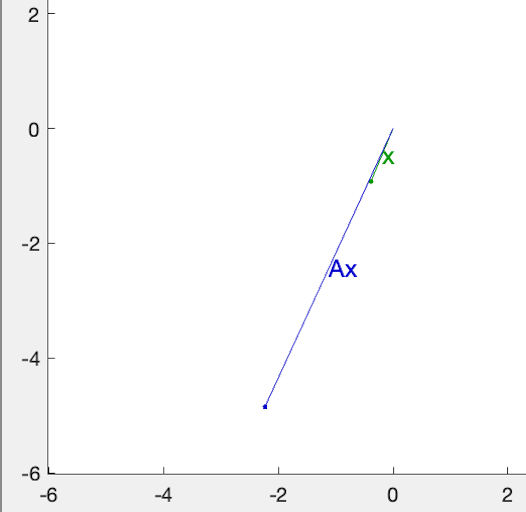
\includegraphics[height=2cm]{pictures/pic1.png} % first figure itself
        \label{fig:figure1}
    \end{minipage}\hfill
    \begin{minipage}{0.45\textwidth}
        \centering
        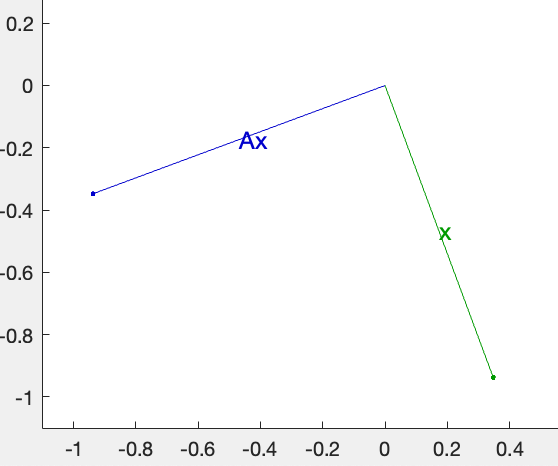
\includegraphics[height=2cm]{pictures/pic3.png} % second figure itself
        \label{fig:figure2}
    \end{minipage}
    \caption{The left image demonstrates~\textbf{x} (green vector) as an eigenvector of matrix \textbf{A}, transforming into \textbf{Ax} (blue vector) as a scaled version of \textbf{x}. 
    The right image shows that the green vector is not an eigenvector of \textbf{A}, as its transformation \textbf{Ax} (blue vector) does not maintain the same direction as \textbf{x}.}
    \label{fig:two_images}
\end{figure}

MATLAB serves as a mediational tool, aligning with Vygotsky's theory which underscores the importance of tool usage and integration in students' developmental processes. As students advance in their linear algebra studies, their engagement with such tools transitions from mere eigenvector computations to a more profound understanding of the underlying mechanics of these computations.

After introducing students to eigenvectors, I present three $10 \times 2$ matrices (referred to as~\textbf{data} and as seen in Figure~\ref{fig:three_images} where I have plotted them) to demonstrate two-dimensional data compression: one matrix with data along the $y=x$ line, another along the $x$ axis, and the third along the $y$ axis. 
The complete MATLAB code is available in the~\ref{appendix:compressionyx} and ~\ref{appendix:compressionx} and~\ref{appendix:compressiony} of this paper.
%In Figure~\ref{fig:three_images}, I plot the data points in the three matrices.
\begin{figure}[ht]
    \centering
    \begin{minipage}{0.32\textwidth}
        \centering
        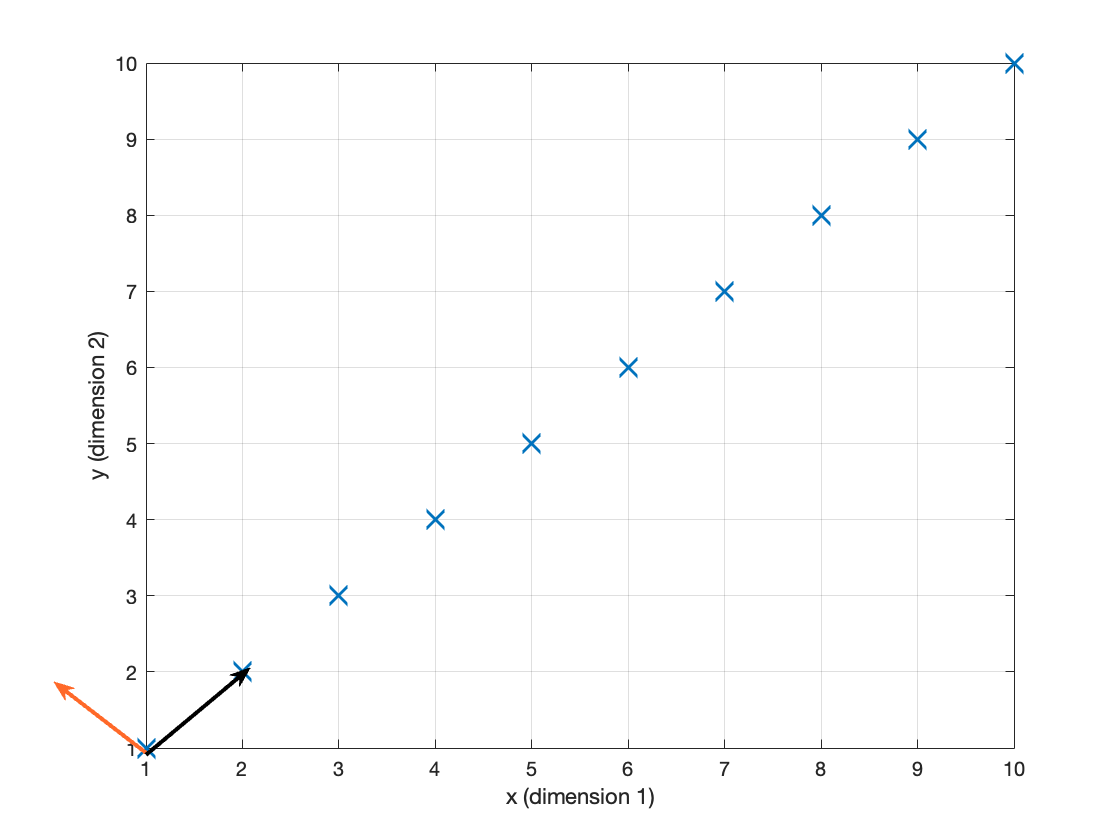
\includegraphics[height=3cm]{pictures/u1.png} % First image
        \label{fig:image1}
    \end{minipage}\hfill
    \begin{minipage}{0.32\textwidth}
        \centering
        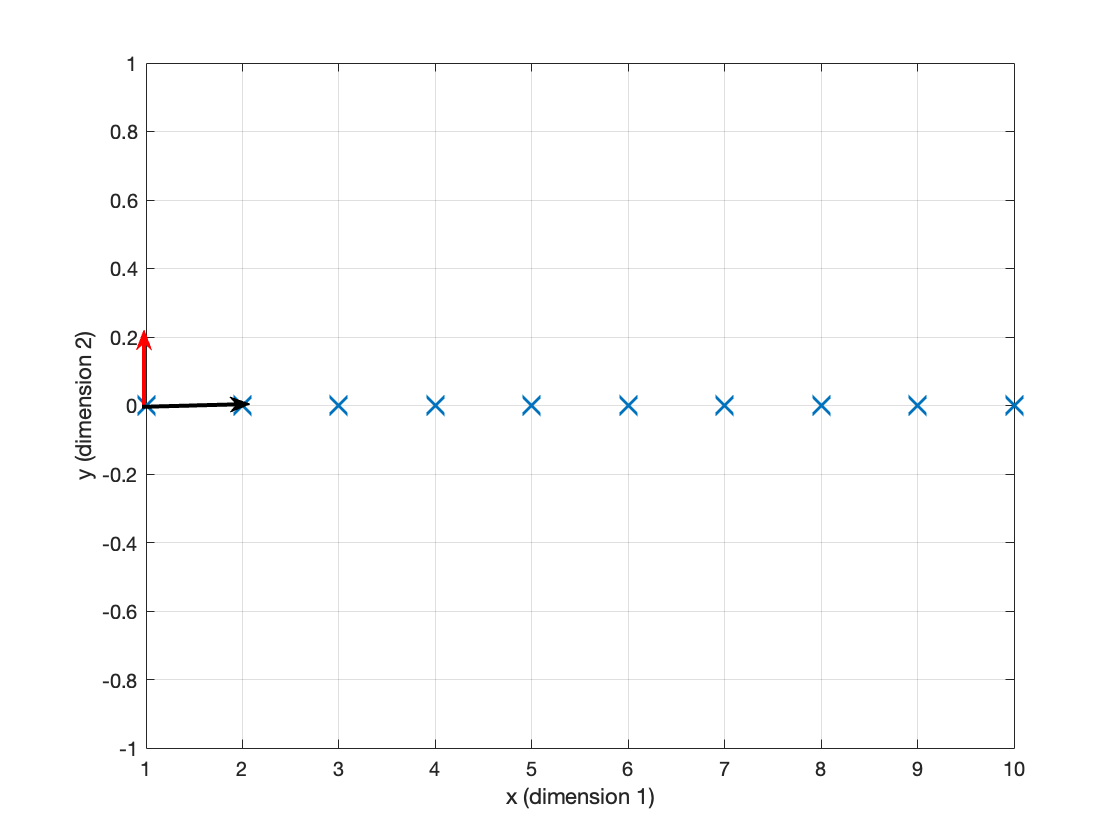
\includegraphics[height=3cm]{pictures/u2.png} % Second image
        \label{fig:image2}
    \end{minipage}\hfill
    \begin{minipage}{0.32\textwidth}
        \centering
        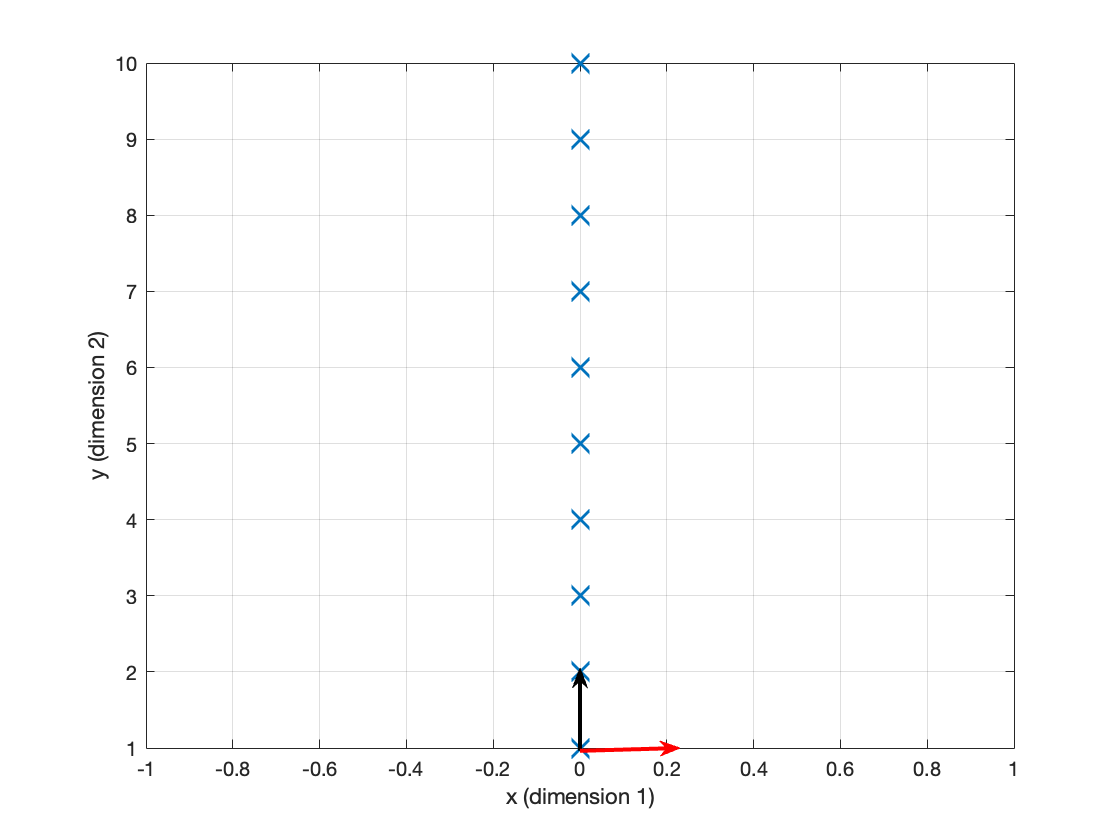
\includegraphics[height=3cm]{pictures/u3.png} % Third image
        \label{fig:image3}
    \end{minipage}
    \caption{First image shows data along the y=x line, the second image displays data along the x-axis, and the third image represents data along the y-axis.}
    \label{fig:three_images}
\end{figure}


The students' task involves identifying the optimal vector for compressing two-dimensional data, as depicted in Figure~\ref{fig:three_images}. 
This figure clearly shows that the best compression vector coincides with the direction of the maximum data spread. 
In the three scenarios presented, this corresponds to along the $y=x$ line, the $x$-axis, and the $y$-axis. 
Through this exercise, students learn that the optimal compression vector not only aligns with the maximum spread but also captures the entire variance of the original data. 
This is visually represented in each plot of Figure~\ref{fig:three_images} by a black arrow, indicating the direction of maximum variance. 
Specifically, the variance is $18.33$ for data along the $y=x$ line and $9.1667$ for data along the $x$ and $y$ axes. 
To quantify this variance, students calculate it either manually or using the $var$ function in MATLAB.

I then encourage my students to create a $2 \times 2$ covariance matrix for each of the three~\textbf{data} matrices. 
In these matrices, the diagonal elements represent the variance along the $x$ and $y$ axes. 
This exercise aids in understanding that the total variance of the~\textbf{data} matrix, which they previously calculated manually or using MATLAB's $var$ function, is equal to the sum of the diagonal elements in the covariance matrix.
The off-diagonal elements are determined by the relationship between the $x$ and $y$ dimensions in each data set. 
The covariance matrix is \( \begin{bmatrix} 9.1667 & 9.1667 \\ 9.1667 & 9.1667 \end{bmatrix} \) when the data points lie along the $y=x$ line. 
Conversely where data points are aligned along the y-axis and x-axis respectively, the covariance matrices are \( \begin{bmatrix} 0 & 0 \\ 0 & 9.1667 \end{bmatrix} \) and \( \begin{bmatrix} 9.1667 & 0 \\ 0 & 0 \end{bmatrix} \).

Computing eigenvectors for these matrices using MATLAB's \texttt{eig} command, students discover that the primary eigenvector (black arrow) aligns with the direction of maximum spread, and its eigenvalue represents the total variance. 
Additionally, they observe a secondary eigenvector (red arrow), perpendicular to the first and indicating zero variance, as evident from its eigenvalue of 0. 
This observation reinforces the understanding that the primary eigenvector captures all the variance of the original data matrix.
The collaborative approach I adopt in my lectures aligns with Vygotsky's scaffolding concept and ZPD.
ZPD is the gap between what a student can do without help and what a student can do with help. 
The initial exercise where students draw the black vector indicating maximum spread now seamlessly integrates with their newfound understanding gained from computing eigenvectors of the covariance matrix. 
This progression illustrates the scaffolding process and helping students through the ZPD, where early, simpler tasks lay the foundation for grasping more complex concepts.

Students often raise two key questions at this juncture: 
(1) Why does computing the eigenvectors of a covariance matrix indicate the direction of maximum spread?
(2) How does this method apply to randomly generated or multi-dimensional data?
In addressing students' queries regarding the covariance matrix and its application to multi-dimensional data, I engage in a collaborative problem-solving process. 
%This approach not only exemplifies Vygotsky's emphasis on social learning and cognitive development through interaction but also encourages students to think critically and independently, key aspects of Piaget's formal operational stage.
To address the first query,
instead of the $10 \times 2$~\textbf{data} matrix from Figure~\ref{fig:three_images}, I now consider 
a mean-adjusted \(n \times d\) matrix referred to as \(\mathbf{data}\). 
Compressed data is defined as \(\mathbf{data_{c}} = \mathbf{data} \times \mathbf{c}\), where \(\mathbf{c}\) is the compression vector and \(\mathbf{data_{c}}\) is the compressed data along the $\mathbf{c}$ vector. 
The goal is to find the compression vector~\textbf{c} that maximize the variance of \(\mathbf{data_{c}}\), given by $\text{Var}(\mathbf{data_{c}}) = \frac{\mathbf{data_{c}}^T \times \mathbf{data_{c}}}{n}$. 
This is similar to the exercise that my students engaged previously with Figure~\ref{fig:three_images} in finding the black vector pointing in the direction of the maximum variance. 
The optimization problem then is to maximize $\mathbf{c^T \times data^T \times data \times c}$, where $\mathbf{data^T \times data}$ represents the covariance matrix \(\mathbf{C}\). 
%Students now realize the relevance of the manually created covariance matrix, which initially appeared random and disconnected. 
%This understanding unfolds as we collaboratively work to maximize the variance of the data along the compressed vector, revealing the seamless and purposeful nature of the covariance matrix in the context of our analysis.
This translates to aligning the vector \(\mathbf{C \times c}\) with the vector \(\mathbf{c}\),indicating that \(\mathbf{c}\) is an eigenvector of \(\mathbf{C}\).
This is because in order to maximize the dot product of the vectors $\mathbf{c}$ and $\mathbf{C}\times \mathbf{c}$ the vector $\mathbf{C}\times \mathbf{c}$ must be in the same direction as $\mathbf{c}$.
Through this interactive and joint exploration, I aim to transition students' understanding from a social plane, where learning is collaborative and external, to a cognitive plane, creating internalization of these concepts. 
This internalization process will be assessed later through individual assignments, allowing me to evaluate each student's independent grasp and application of the learned material.

For the second question, I use a \(360 \times 640\) grayscale image as the \(\mathbf{data}\) matrix. 
The complete MATLAB code is available in~\ref{appendix:compressionbu} of this paper. 
\begin{figure}[H]
    \centering
    \begin{minipage}{0.18\textwidth}
        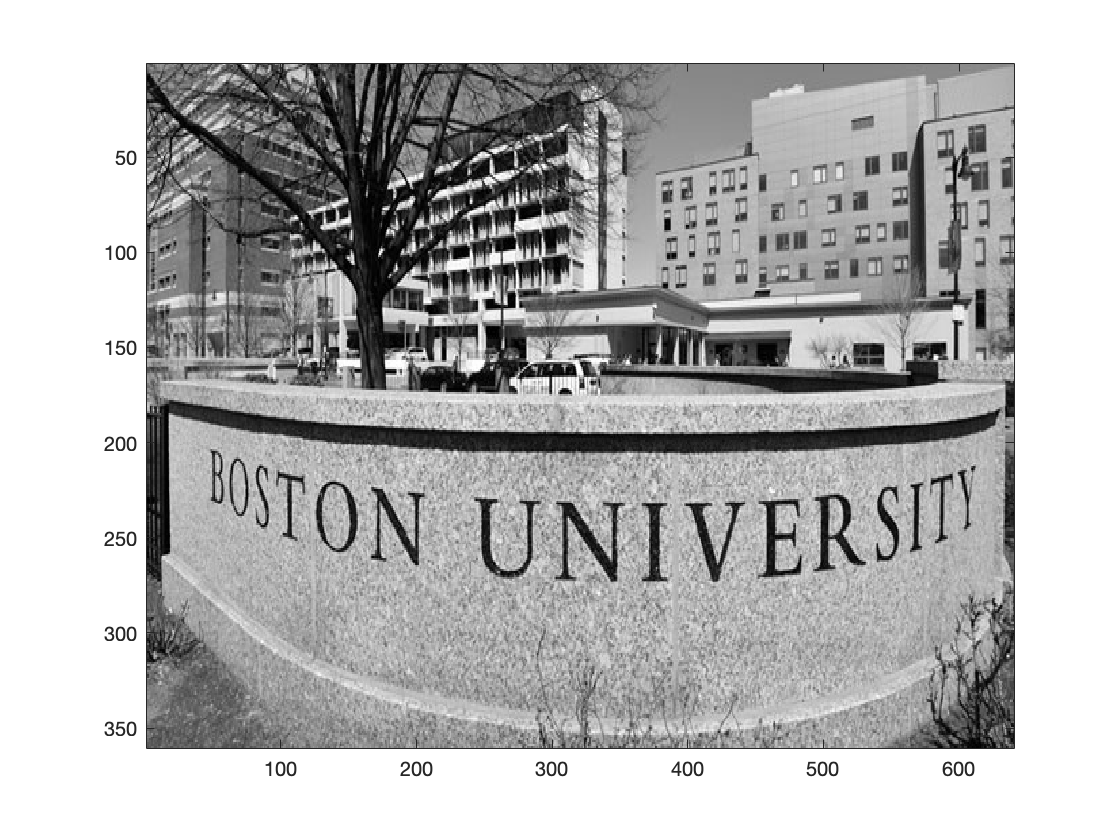
\includegraphics[width=\linewidth]{pictures/compression0.png}
        \label{fig:image11}
    \end{minipage}
    \hfill
    \begin{minipage}{0.18\textwidth}
        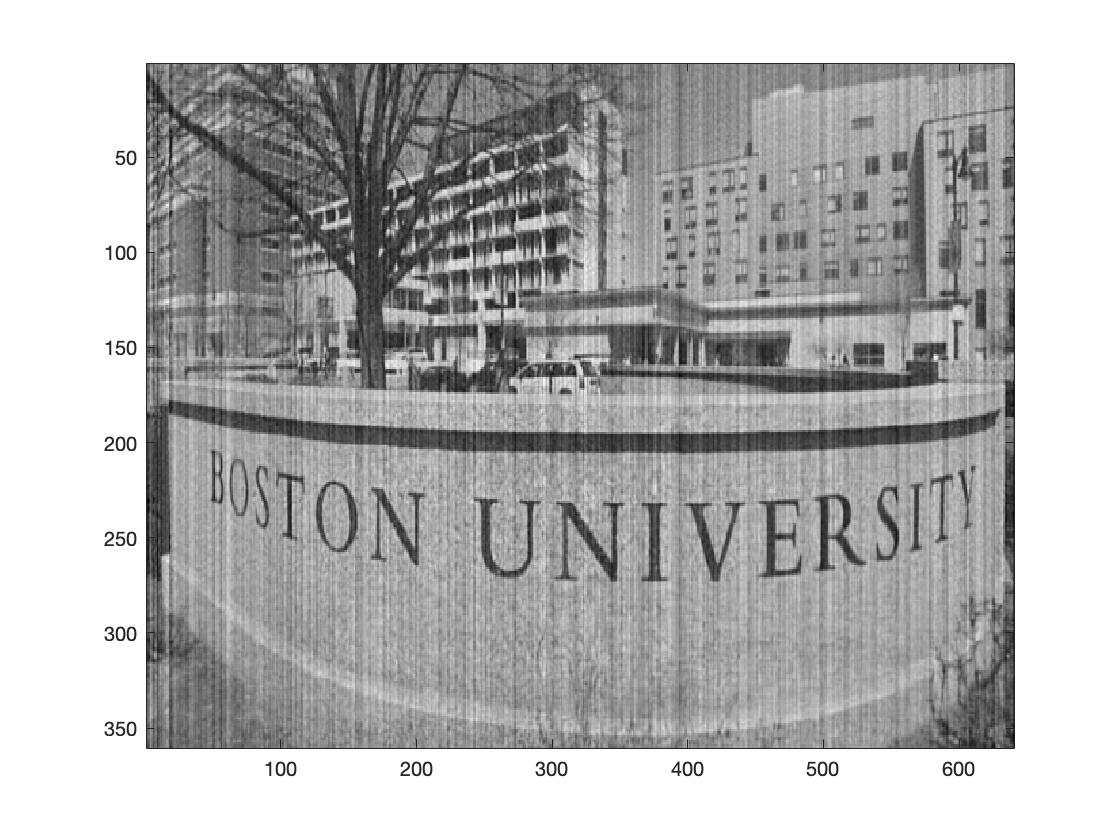
\includegraphics[width=\linewidth]{pictures/compression1.png}
        \label{fig:image21}
    \end{minipage}
    \hfill
    \begin{minipage}{0.18\textwidth}
        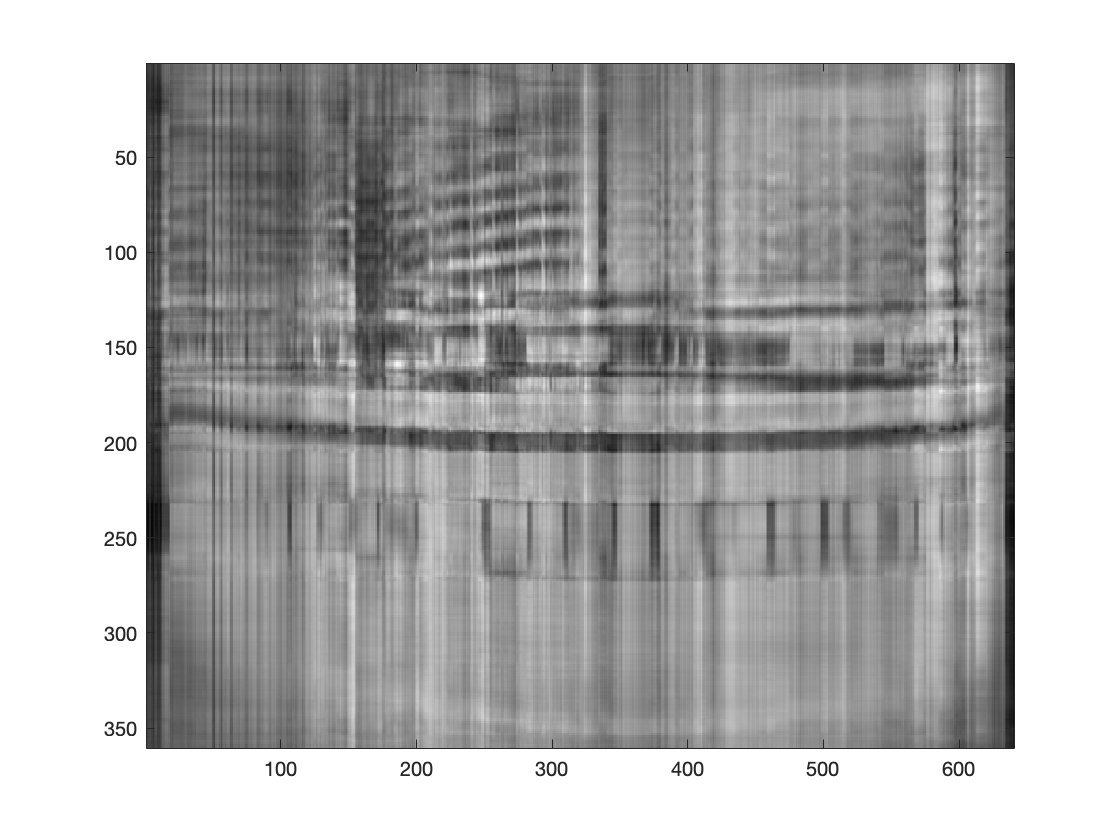
\includegraphics[width=\linewidth]{pictures/compression2.png}
        \label{fig:image31}
    \end{minipage}
    \hfill
    \begin{minipage}{0.18\textwidth}
        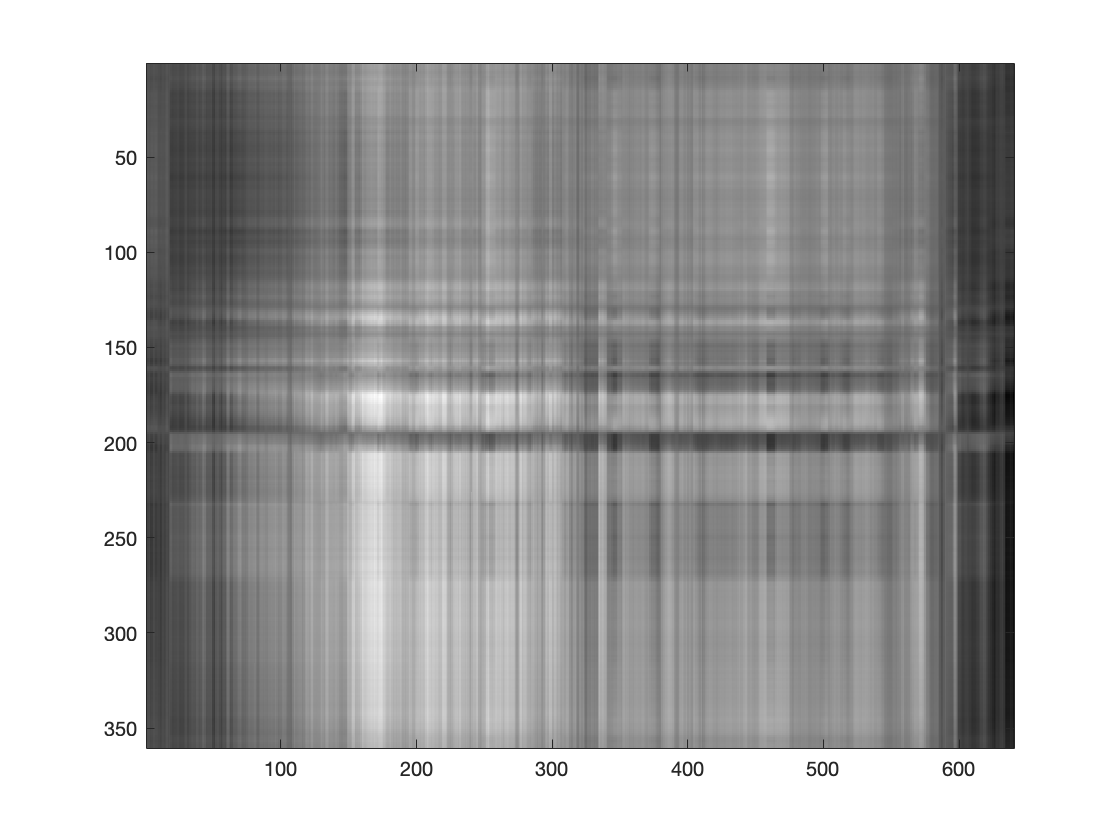
\includegraphics[width=\linewidth]{pictures/compression4.png}
        \label{fig:image41}
    \end{minipage}
    \hfill
    \begin{minipage}{0.18\textwidth}
        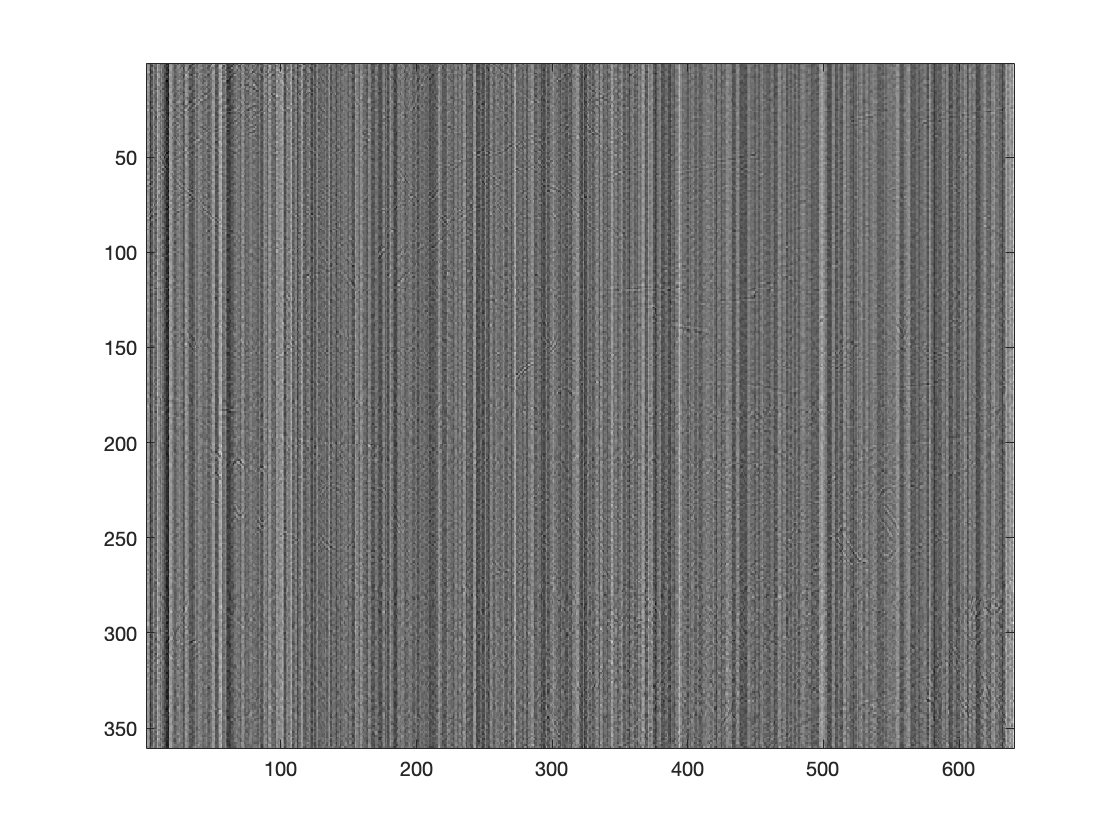
\includegraphics[width=\linewidth]{pictures/compression5.png}
        \label{fig:image51}
    \end{minipage}
    \caption{Grayscale Image Compression: Original image and its compressed versions using the 100 largest, 30 largest, 1 largest, and 500 smallest eigenvectors.}
    \label{fig:five_images}
\end{figure}
Students observe from Figure~\ref{fig:five_images} the effects of image compression using different numbers of eigenvectors.
What my students are truly amazed by is that there is very little to no variance captured by the 500 smallest eigenvectors (based on their eigenvalues). 
These visual examples highlight the importance of variance preservation and demonstrate that discarding eigenvectors with minimal variance has a negligible impact on image quality and can lead to higher compression without losing much of the information captured in the picture.
This hands-on MATLAB experience provides students with a concrete understanding of linear algebra concepts, as they visualize the practical effects of image compression with different numbers of eigenvectors.

As students observe and discuss the outcomes of different compression levels, they are engaging in a social learning process, which then transitions into individual understanding and cognitive development. 
The use of MATLAB as a mediational tool in this experiment not only simplifies the complex concept of dimensional reduction in PCA but also makes the learning experience more engaging and relatable. 
This process, aligning with Vygotsky's educational theory, transitions learning from a social context – collaborative discussions and guided exploration in the classroom – to internal cognitive processing. 
%This aligns perfectly with Vygotsky's emphasis on the role of social interaction and practical tools in learning, thereby enhancing the students' ability to internalize and apply the mathematical concepts of linear algebra in a meaningful way.

\section{Conclusions}
\label{sec:conclusion}
In conclusion, integrating Vygotsky's theory into linear algebra teaching fosters an engaging, collaborative, and effective learning environment, crucial for students' mastery and application of the subject.

\section*{Acknowledgement}
I gratefully acknowledge the use of OpenAI's ChatGPT for proofreading, grammatical checks, and other text editing tasks.
%I also like to thank all the wonderful administrative staff, teachers and students at Boston University Academy that assisted me during the gaming workshop. 

\medskip

\printbibliography

\appendix
% To ensure the appendices are not just another section
\renewcommand{\thesection}{Appendix \Alph{section}}

\section{MATLAB Code for compression along the y=x line}
\label{appendix:compressionyx}
\begin{lstlisting}
%compression on Y=X line
x = 1:10;
y = x;
plot(x, y, 'X', 'MarkerSize', 10, 'LineWidth', 2)
xlabel('x (dimension 1)')
ylabel('y (dimension 2)')
grid on
data=[x' y']
[V,D]=eig(cov(data))
% Compute the mean of data
meanData = mean(data);

% Scale factor for the eigenvectors
scaleFactor = 5;

% Plotting the scaled eigenvectors
hold on; % Keep the current plot
quiver(meanData(1), meanData(2), scaleFactor * V(1,1), scaleFactor * V(2,1), 'r'); % First eigenvector
quiver(meanData(1), meanData(2), scaleFactor * V(1,2), scaleFactor * V(2,2), 'k'); % Second eigenvector
hold off;

\end{lstlisting}

\section{MATLAB Code for compression along the X axis}
\label{appendix:compressionx}
\begin{lstlisting}
%compression on X axis
x = 1:10;
y = zeros(1,10);
plot(x, y, 'X', 'MarkerSize', 10, 'LineWidth', 2) 
xlabel('x (dimension 1)')
ylabel('y (dimension 2)')

grid on
data=[x' y']
[V,D]=eig(cov(data))
% Compute the mean of data
meanData = mean(data);

% Scale factor for the eigenvectors
scaleFactor = 5;

% Plotting the scaled eigenvectors
hold on; % Keep the current plot
quiver(meanData(1), meanData(2), scaleFactor * V(1,1), scaleFactor * V(2,1), 'r'); % First eigenvector
quiver(meanData(1), meanData(2), scaleFactor * V(1,2), scaleFactor * V(2,2), 'k'); % Second eigenvector
hold off;

\end{lstlisting}


\section{MATLAB Code for compression along the Y axis}
\label{appendix:compressiony}
\begin{lstlisting}
%compression on Y axis
y = 1:10;
x = zeros(1,10);
plot(x, y, 'X', 'MarkerSize', 10, 'LineWidth', 2) 
xlabel('x (dimension 1)')
ylabel('y (dimension 2)')
grid on
data=[x' y']
[V,D]=eig(cov(data))
% Compute the mean of data
meanData = mean(data);

% Scale factor for the eigenvectors
scaleFactor = 5;

% Plotting the scaled eigenvectors
hold on; % Keep the current plot
quiver(meanData(1), meanData(2), scaleFactor * V(1,1), scaleFactor * V(2,1), 'r'); % First eigenvector
quiver(meanData(1), meanData(2), scaleFactor * V(1,2), scaleFactor * V(2,2), 'k'); % Second eigenvector
hold off;

\end{lstlisting}

\section{Noisy Image Compression}
\label{appendix:compressionbu}
\begin{lstlisting}
%compression on BU.jpg example
img_in=double((rgb2gray(imread('BU.jpg'))));
numberOfDataPoints=size(img_in,1);
numberOfDimensions=size(img_in,2);
numberOfEigenVectors=100
imagesc(img_in);
colormap(gray);  % Set the colormap to grayscale
[V,D]=eig(cov(img_in))
imagesc((V(:,numberOfDimensions-numberOfEigenVectors:numberOfDimensions)*V(:,numberOfDimensions-numberOfEigenVectors:numberOfDimensions)'*img_in')')
\end{lstlisting}
\end{document}


